\begin{frame}{Phänomenologie}
\textbf{Supraleitung}: Ab einer Sprungtemperatur $T_{\mathup{C}}$ fällt elektrischer Widerstand auf $\SI{0}{\ohm}$ \\
\begin{columns}
\begin{column}{0.49\textwidth}
  \begin{figure}
    \fbox{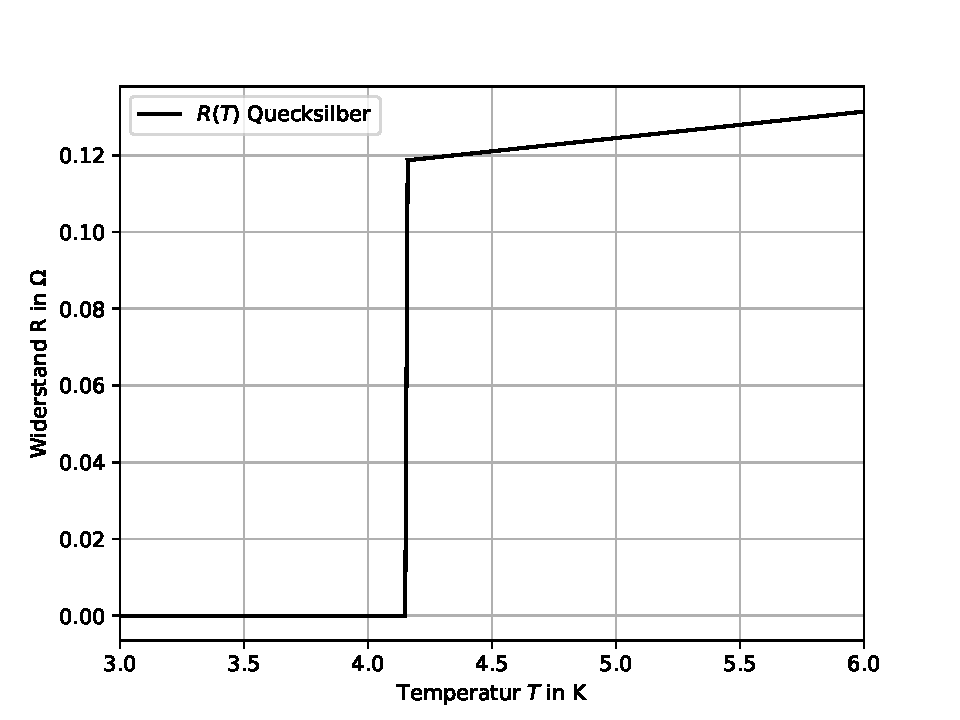
\includegraphics[width = \textwidth]{quecksilber_supra.pdf}}
    \label{fig: hg_supraleitung}
  \end{figure}
\end{column}
\begin{column}{0.49\textwidth}

\begin{table}
  \caption{Sprungtemperaturen \cite{dem2}}
  \label{tab: sprungtemperaturen}
\begin{tabular}{l S}
  & $T_{\mathup{C}} / \si{\kelvin}$ \\
  \text{Queksilber} & \num{4.15} \\
    \text{Aluminium} & \num{1.17} \\
      \text{\ce{TlCaBaCuO}} & \num{125}
\end{tabular}
\end{table}
\end{column}
\end{columns}
\end{frame}



\begin{frame}{Meißner-Ochsenfeld-Effekt}
\begin{columns}
\begin{column}{0.49\textwidth}
  \begin{figure}
    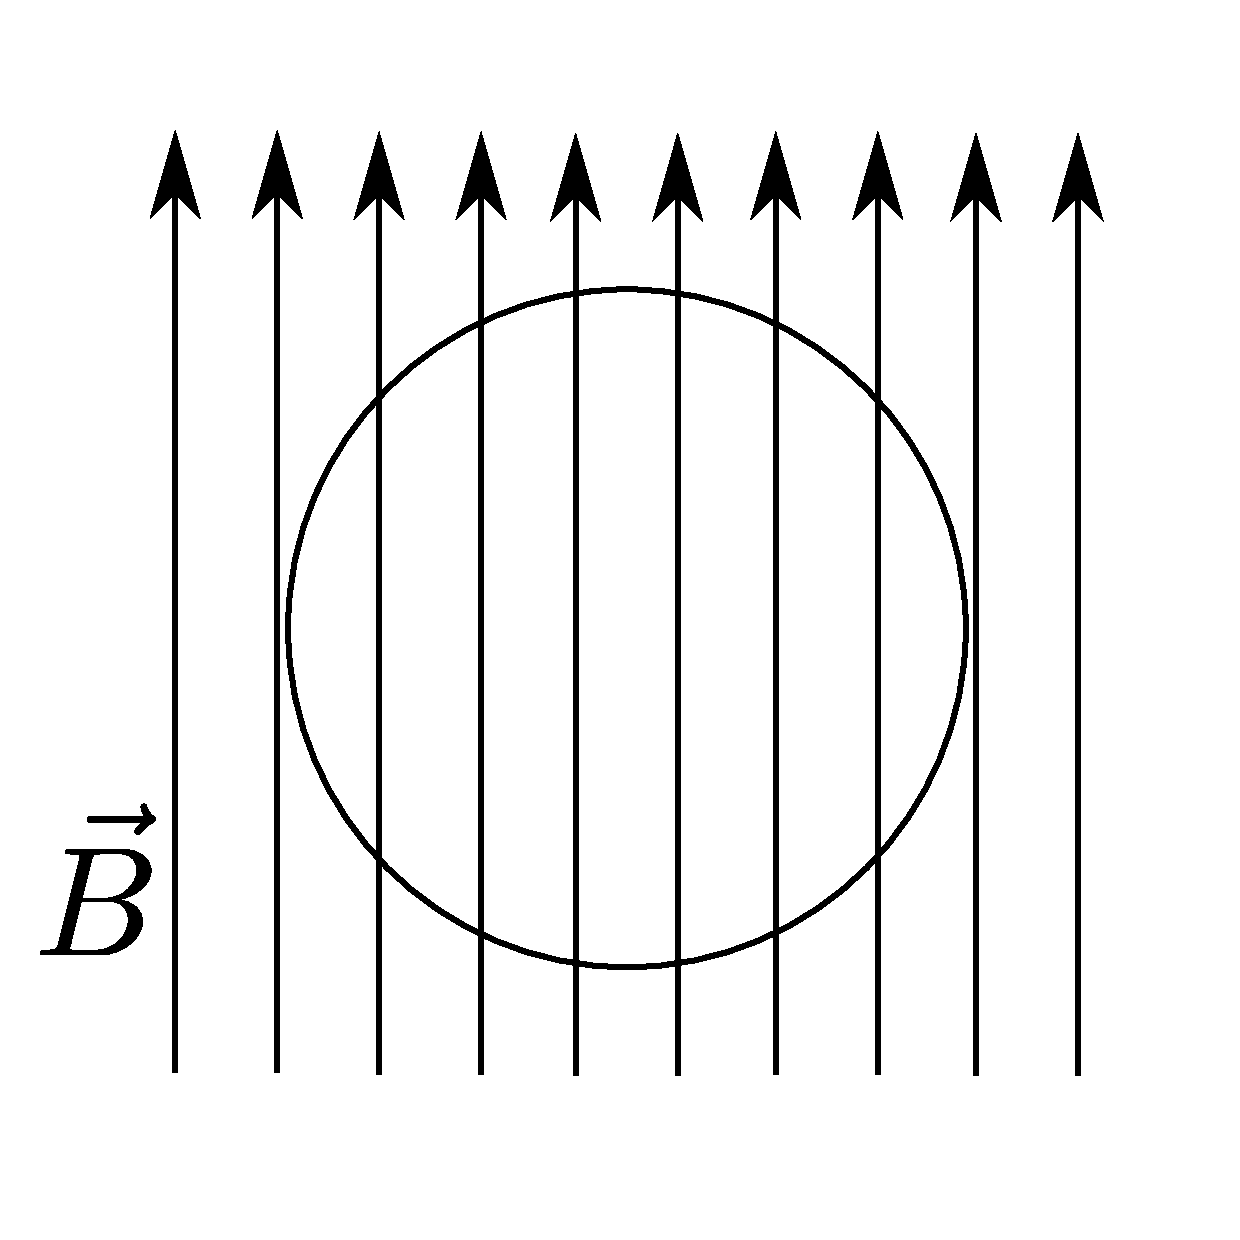
\includegraphics[width = \textwidth]{supra_1.pdf}
    \caption{Normale Leitung $T > T_{C}$}
    \label{fig: bfeld_normale_leitung}
  \end{figure}
\end{column}
\begin{column}{0.49\textwidth}
  \begin{figure}
    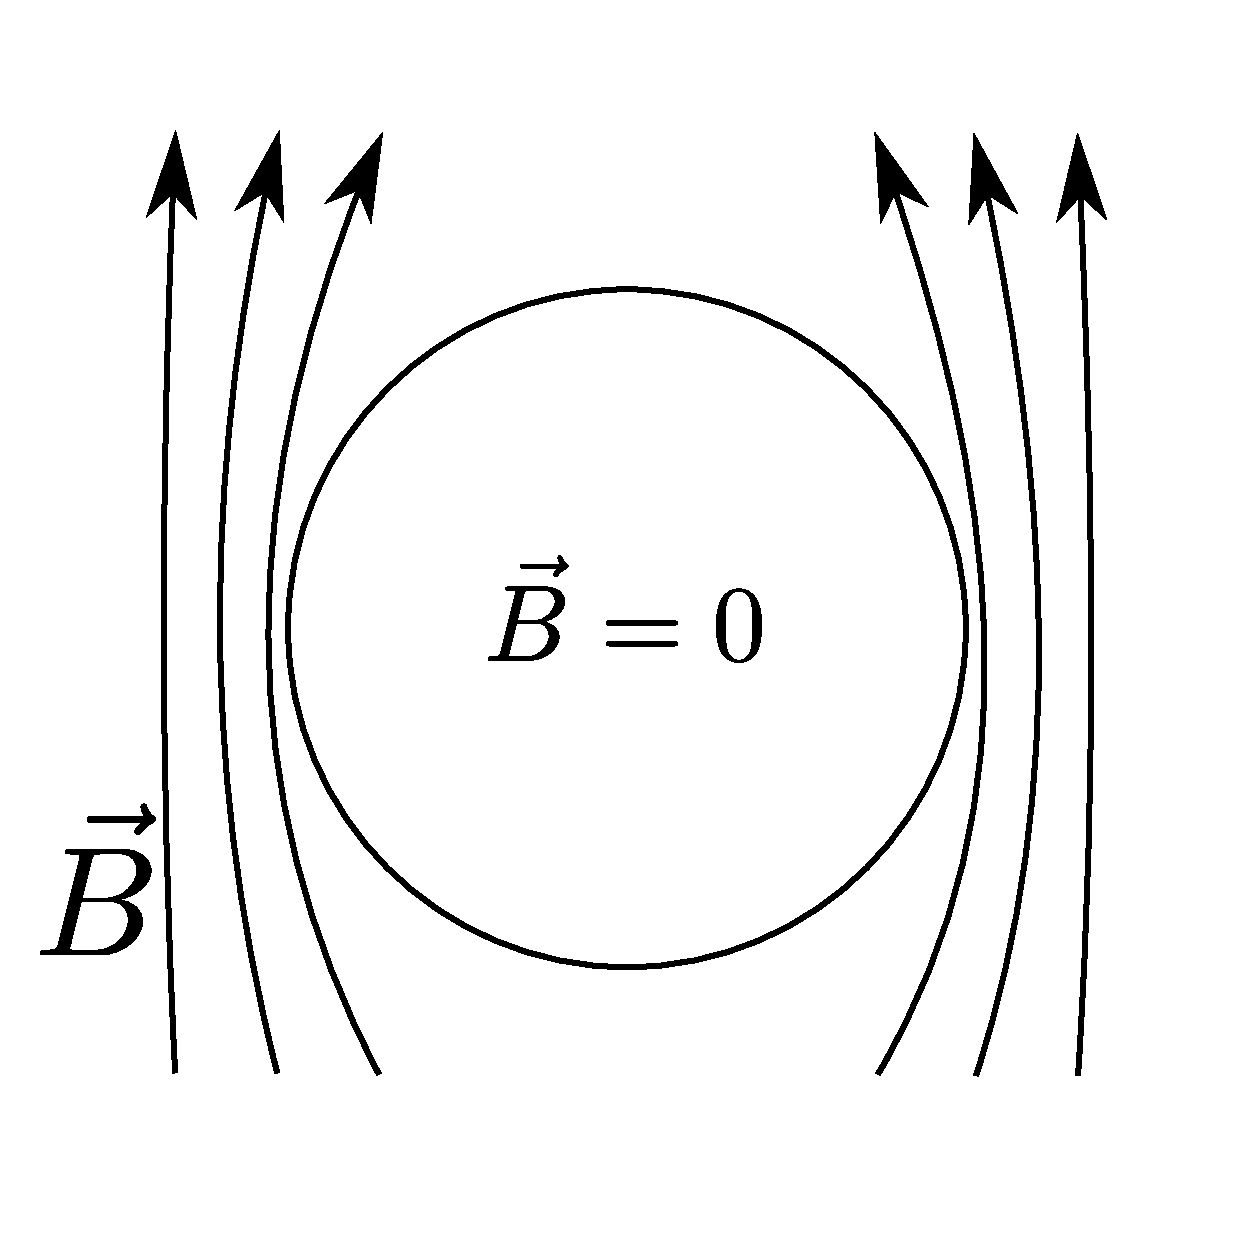
\includegraphics[width = \textwidth]{supra_2.pdf}
    \caption{Supraleitung $T < T_{C}$}
    \label{fig: bfeld_supraleitung}
  \end{figure}
\end{column}
\end{columns}
\end{frame}
